\chapter{Weitere Prinzipien}
General Responsibility Assignment Software Patterns (GRASP) sind eine Sammlung von Prinzipien, welche in der Softwareentwicklung verwendet werden. In diesem Kapitel werden die Prinzipien Geringe Kopplung und Hohe Kohäsion vorgestellt. Außerdem wird das Prinzip Don't Repeat Yourself (DRY) vorgestellt.
\section{Analyse GRASP: Geringe Kopplung}
% jeweils eine bis jetzt noch nicht behandelte Klasse als positives und negatives Beispiel geringer Kopplung; jeweils UML Diagramm mit zusammenspielenden Klassen, Aufgabenbeschreibung und Begründung für die Umsetzung der geringen Kopplung bzw. Beschreibung, wie die Kopplung aufgelöst werden kann
Low Coupling bezeichnet eine geringe Kopplung zwischen Klassen. Eine geringe Kopplung zwischen Klassen bedeutet, dass eine Klasse nur auf wenige andere Klassen angewiesen ist. Eine Klasse, die auf viele andere Klassen angewiesen ist, ist schwieriger zu warten und zu erweitern. Außerdem ist es schwieriger, die Funktionalität einer Klasse zu testen, wenn diese auf viele andere Klassen angewiesen ist. Zusätzlich lässt sie sich einfacher tauschen oder ersetzen. 
\newpage
\subsection{Positiv-Beispiel}
Ein Beispiel, bei dem das Prinzip der Geringen Kopplung umgesetzt wurde ist die Klasse FlandersHome als Beispiel für die verschiedenen Klassen aus dem Package Homes, welche die Wohnungen der Simpsons Figuren repräsentiert. Wie in Abbildung \ref{fig:flandersHome} zu sehen ist, ist die Klasse FlandersHome nur von der Klasse Home abhängig. Zusätzlich implementiert sie notwendige Methoden des HomeFeature Interfaces. Gibt es beispielsweise eine Änderung am Heim von Rektor Skinner, betrifft es diese Klasse nicht.  
\begin{figure}[ht]
    \centering
    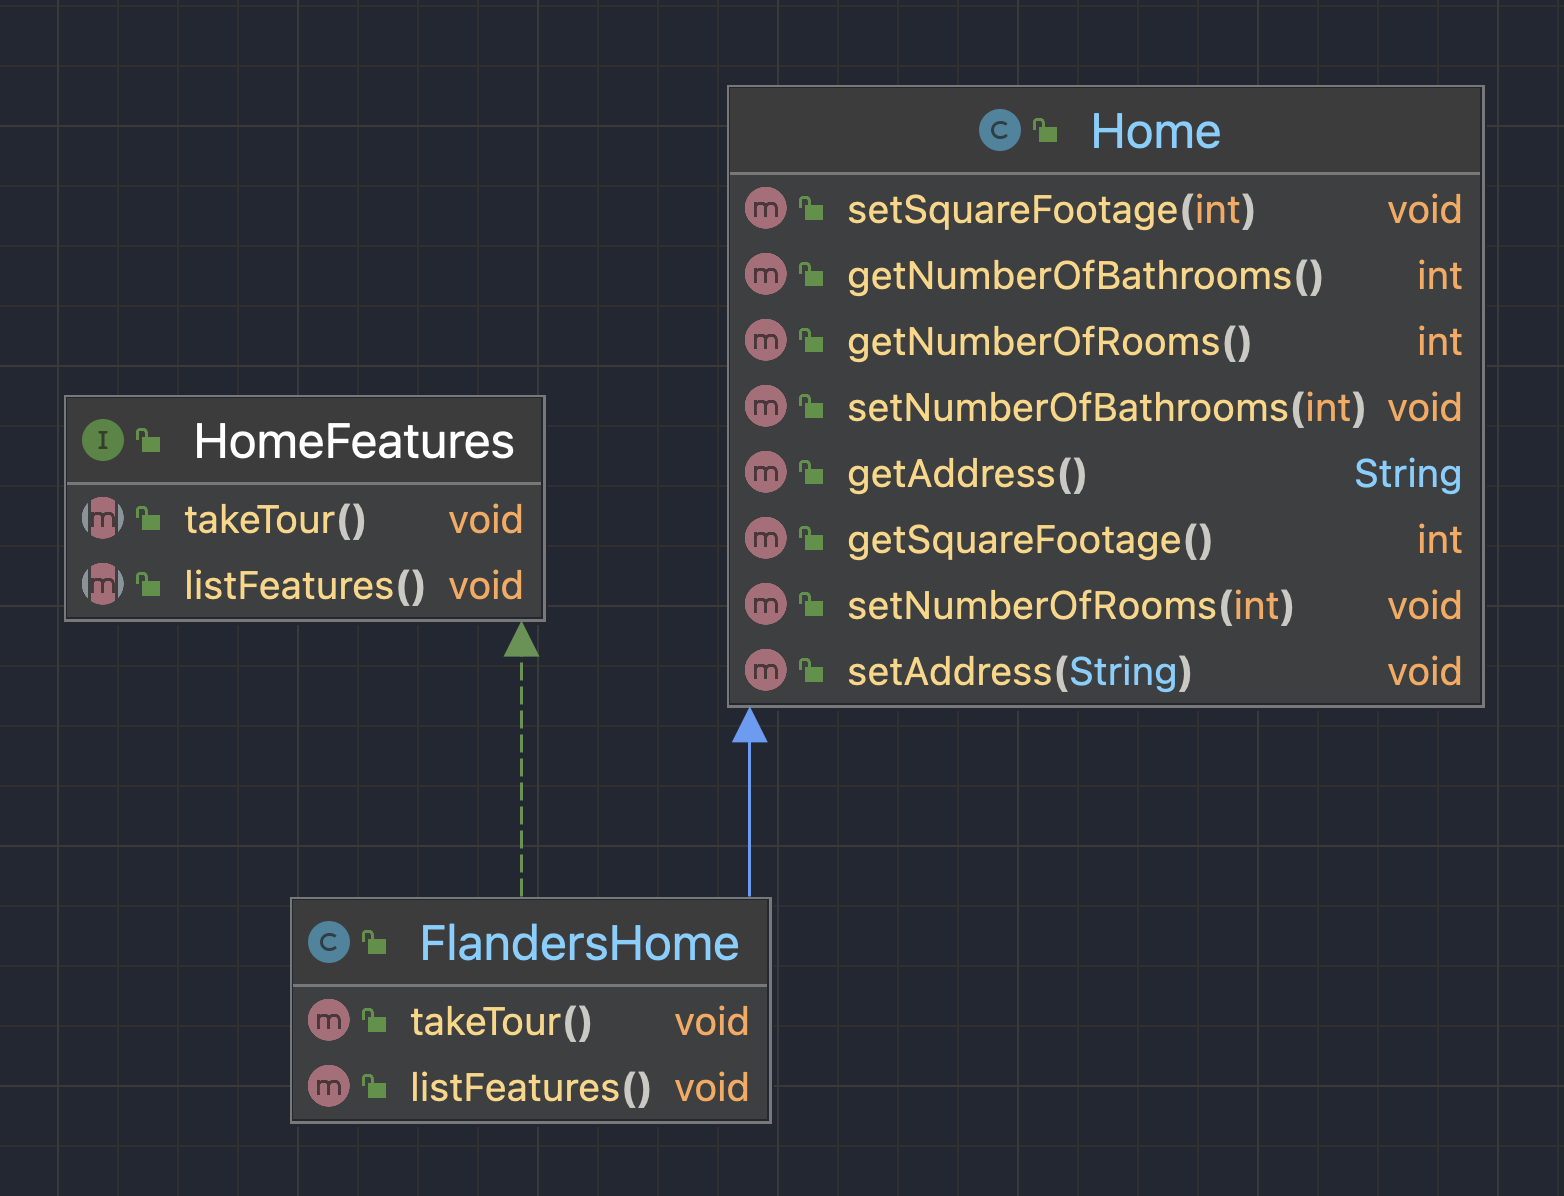
\includegraphics[width=0.3\textwidth]{Bilder/homeI.png}
    \caption{UML Klassendiagramm (FlandersHome) im Zusammenspiel mit Interface}
    \label{fig:flandersHome}
\end{figure}

\subsection{Negativ-Beispiel}
Führt man das zuvor genannte Beispiel eine Ebene nach oben, wird allerdings deutlich, dass die Klasse QuestionManager von jeder Klasse, welche eine der Simpsons Figuren repräsentiert, abhängig ist und somit eine hohe Kopplung aufweist. Abbildung \ref{fig:hoheK} zeigt die Klasse QuestionManager im Zusammenspiel mit den Klassen aus dem Package der Charaktere. 
\begin{figure}[ht]
    \centering
    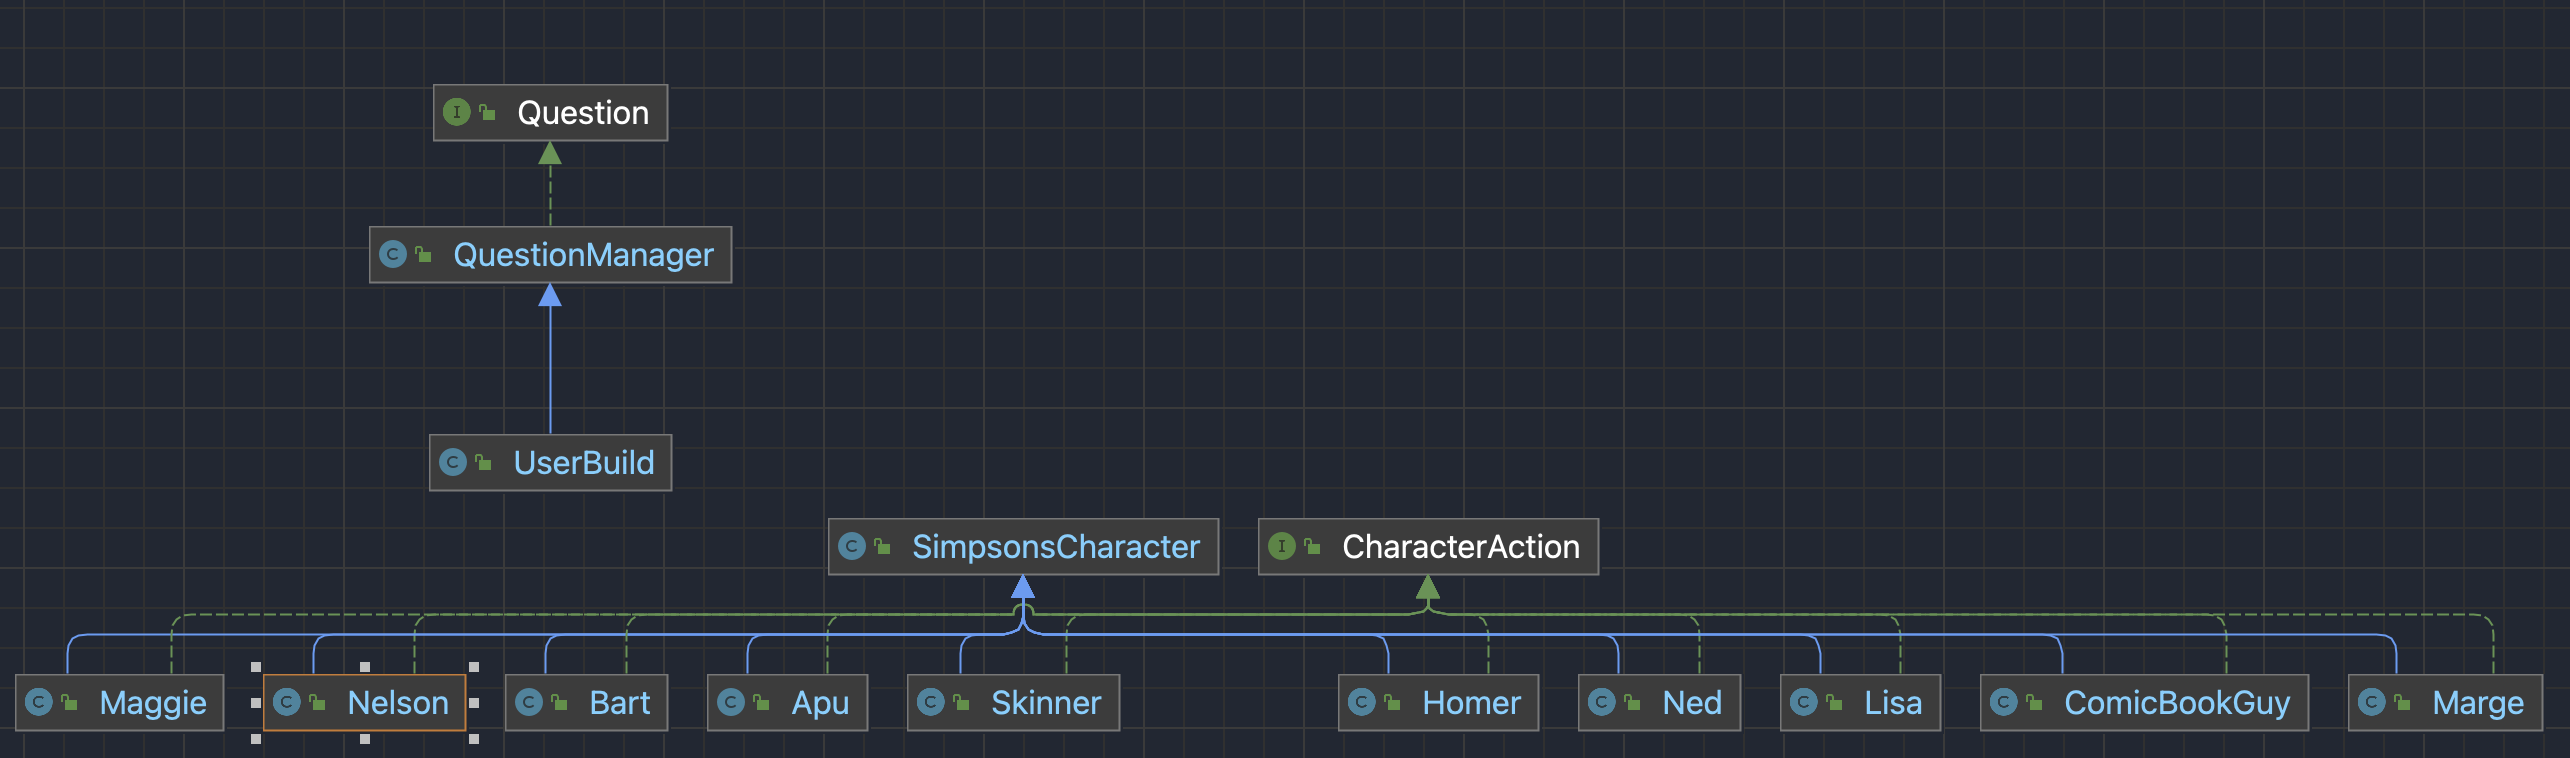
\includegraphics[width=0.8\textwidth]{Bilder/hoheK.png}
    \caption{UML Klassendiagramm (QuestionManager) in Abhängigkeit der Charaktere}
    \label{fig:hoheK}
\end{figure}

\section{Analyse GRASP: Hohe Kohäsion}
% eine Klasse als positives Beispiel hoher Kohäsion; UML Diagramm und Begründung, warum die Kohäsion hoch ist
Hohe Kohäsion ist wichtig, da Objekte so organisiert werden sollten, dass die Methoden und Attribute zusammengehören und eine klar definierte Aufgabe erfüllen. Zusätzlich erhöht es wesentlich die Überschaubarkeit und des Codes. Abbildung \ref{fig:highK} zeigt die Klassen der einzelnen Figuren im Zusammenhang mit ihren Arbeitsstätten und Wohnorte.
\begin{figure}[ht]
    \centering
    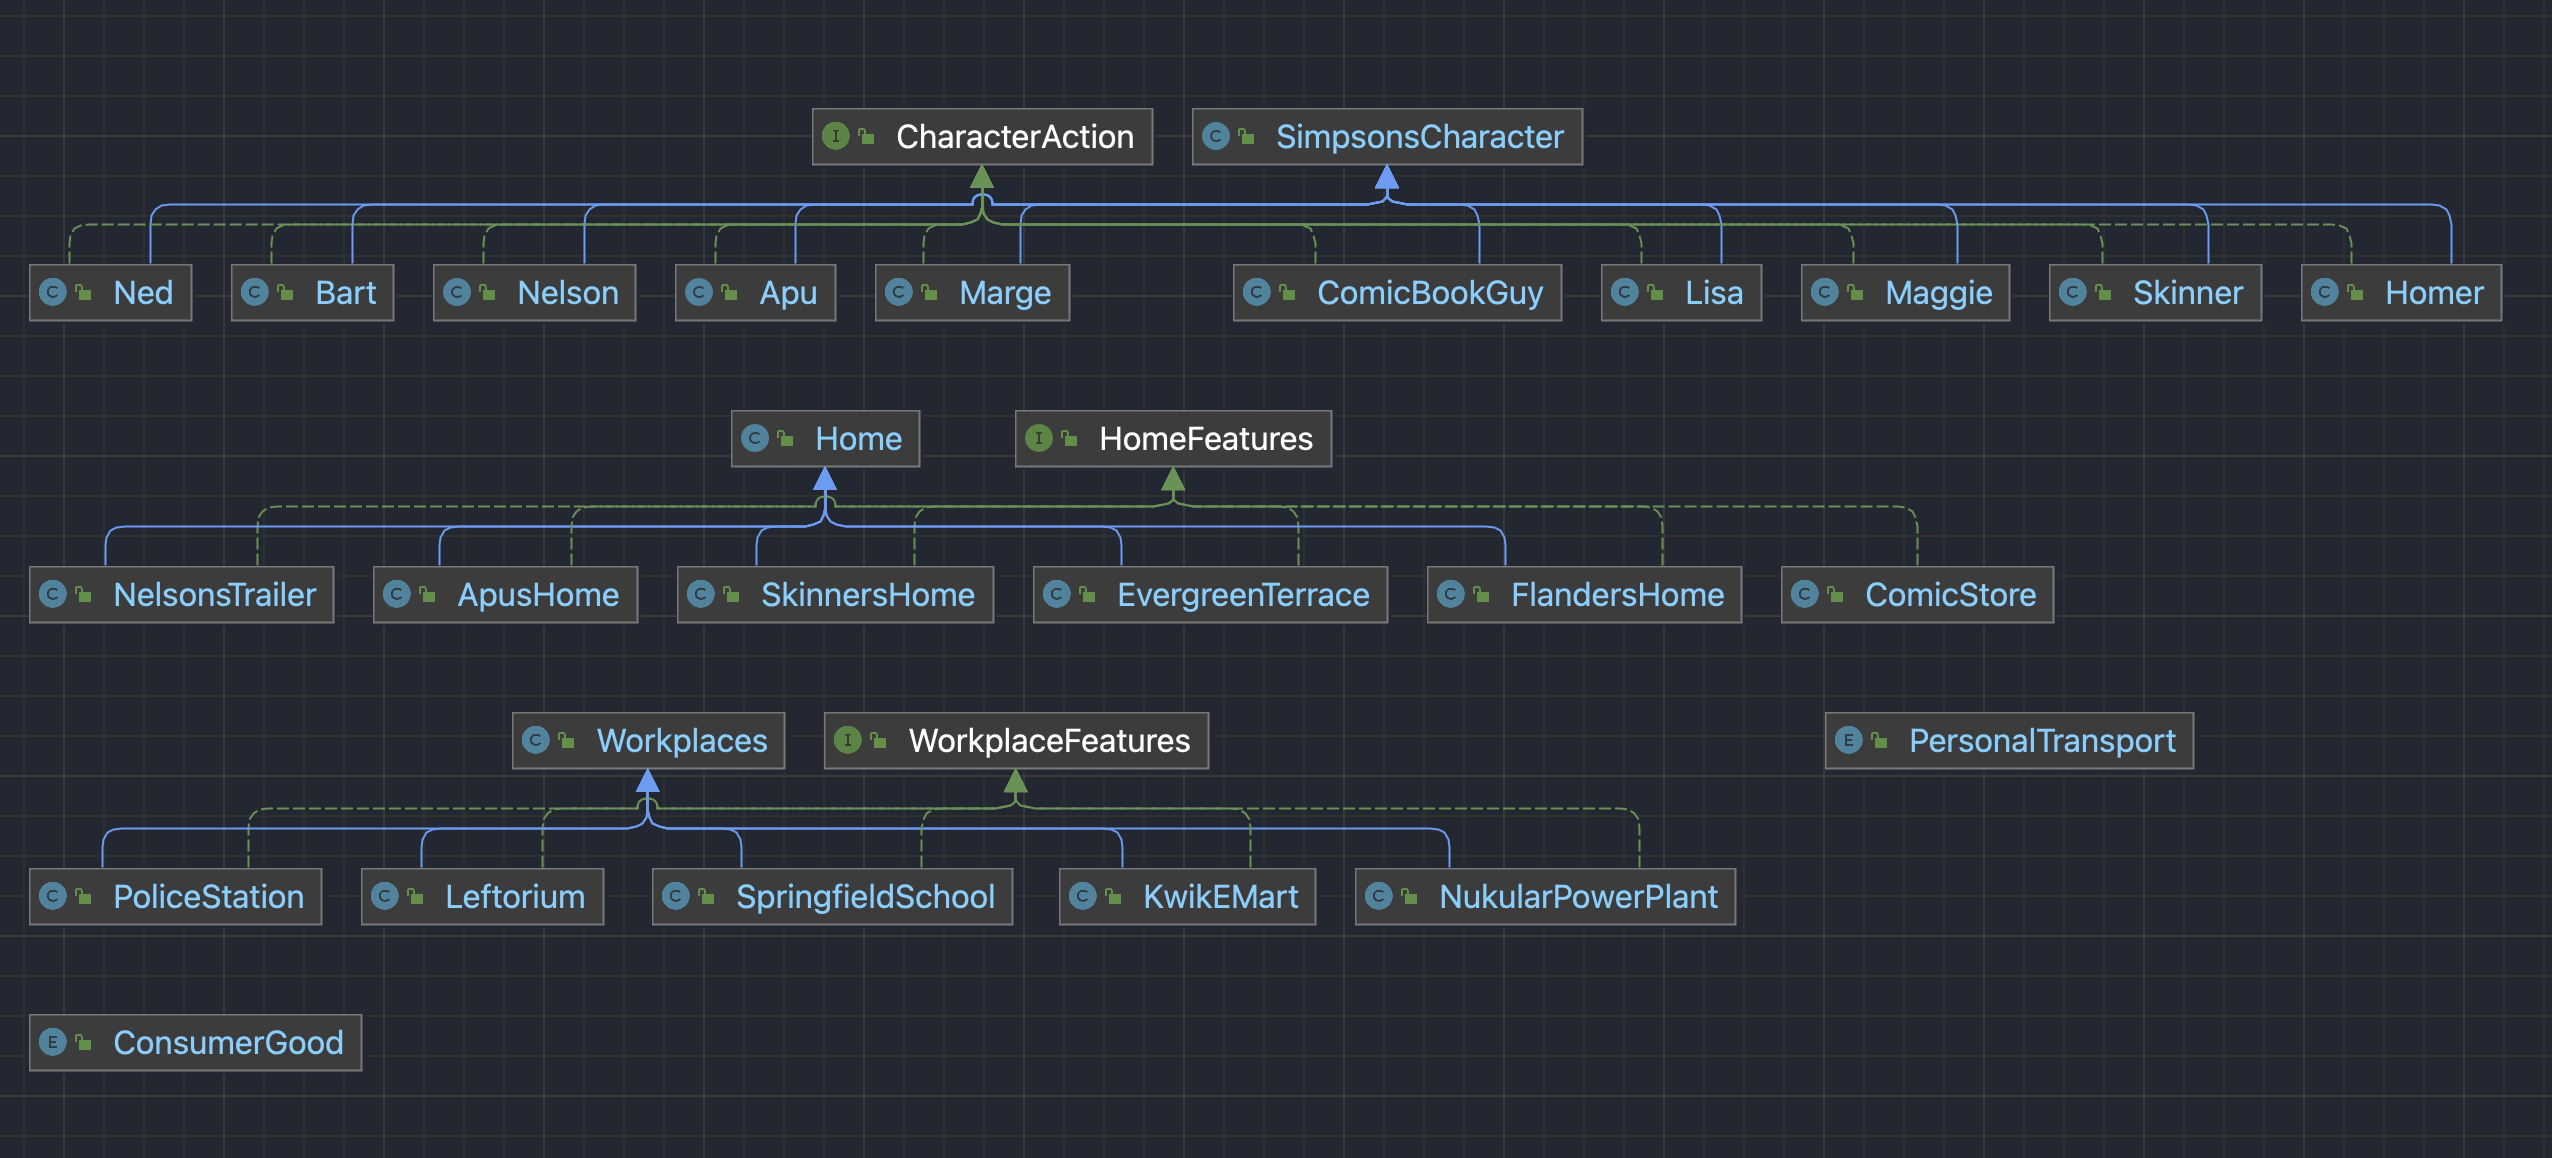
\includegraphics[width=0.8\textwidth]{Bilder/highK.png}
    \caption{UML Klassendiagramm (Charaktere im Zusammenspiel mit Arbeitsstätte und Zuhause)}
    \label{fig:highK}
\end{figure}
\newpage

\section{Don't Repeat Yourself (DRY)}
% ein Commit angeben, bei dem duplizierter Code/duplizierte Logik aufgelöst wurde; Code-Beispiele (vorher/nachher); begründen und Auswirkung beschreiben
DRY ist ein Akronym für Don't Repeat Yourself und ein weiteres Prinzip der Softwareentwicklung. Es bedeutet, dass jede Funktionalität oder Information in einem Programm nur einmal definiert werden sollte um Redundanzen zu vermeiden. So kann beispielsweise Code ausgelagert werden um ihn wiederverwenden zu können ohne ihn zu duplizieren. Außerdem wird die Wartbarkeit des Codes erhöht, da Änderungen nur an einer Stelle vorgenommen werden müssen. So wurde beispielsweise, wie in Listing \ref{code:DRY} zu sehen ist, der Code für die Ausgabe der Charakter Bilder in die SimpsonsCharacter Klasse ausgelagert und kann so direkt von den jeweiligen Klassen aufgerufen werden.
\lstinputlisting[
    label={code:DRY},  % Label; genutzt für Referenzen auf dieses Code-Beispiel
	caption={DRY Prinzip bei Ausgabe der Charakter Bilder},  % Caption; genutzt für Referenzen auf dieses Code-Beispiel
	captionpos=b,               % Position, für die Caption:  t(op) oder b(ottom)
	style=EigenerJavaStyle,     % Eigener Style der vor dem Dokument festgelegt wurde
	firstline=1,                % Zeilennummer im Dokument welche als erste angezeigt wird
	lastline=10     
]{Quellcode/Picture.java}